\documentclass[twoside,numberorder]{csbachelor}

%==============================================================
%==============================================================

\usepackage{url}
\usepackage{subfigure}

% 张海:其他引用
\usepackage[hidelinks]{hyperref}
\setlength{\LTpre}{1em}
\setlength{\LTpost}{1em}

\usepackage{tikz}
\usetikzlibrary{arrows,backgrounds,fit,shapes}
\tikzstyle{layer} = [draw, dashed]
\tikzstyle{block} = [draw, rectangle, minimum height=2em]
\tikzset{>=latex}

% 一些全局工具的定义
\DeclareMathOperator*{\argmin}{arg\,min}
\DeclareMathOperator*{\argmax}{arg\,max}

%==============================================================
%==============================================================

\begin{document}

%==============================================================
%==============================================================

  % 论文题目:{中文}{英文}
  \zjutitle{标题}
           {Title}
  % 作者:{中文姓名}{英文}{学号}
  \zjuauthor{姓名}{Name}{313XXXXXXXX}
  % 指导教师:{导师中文名}{导师英文名}
  \zjumentor{导师姓名}{Supervisor name}
  % 个人信息:{年级}{专业名称}
  \zjuinfo{2013级}{计算机科学与技术}{Computer Science and Technology}
  % 学院信息:{学院中文}{学院英文}
  \zjucollege{计算机科学与技术学院}{College of Computer Science and Technology}
  % 日期:{提交日期}{Submitted Date}
  \zjudate{2017 年 6 月 5 日}{June 5, 2017}

%==============================================================

  {
    \pagestyle{empty}

    {
  \setlength{\parindent}{0em}

  {
    \linespread{1}

    \vspace*{-1em}

    \begin{center}
      
\includegraphics[width=108mm]{data/cover-zh/xiaoming}
    \end{center}

    \vspace{-1.5em}

    {
      \songti\erhao\bfseries
      \centering
      本~~科~~生~~毕~~业~~设~~计 \par
    }

    \vspace{1em}

    \begin{center}
      
\includegraphics[width=35mm]{data/cover-zh/xiaobiao}
    \end{center}
  }

  \vspace{9em}

  {
    \linespread{1.6}
    \songti\sanhao\bfseries
    \centering
    \newlength{\titlelength}
    \setlength{\titlelength}{22em}
    题目 \; \underline{\makebox[\titlelength]{\zjutitlec}} \\
    姓名 \; \underline{\makebox[\titlelength]{\zjuauthornamec}} \\
    学号 \; \underline{\makebox[\titlelength]{\zjuauthorid}} \\
    指导教师 \; \underline{\makebox[\titlelength - 2em]{\zjumentorc}} \\
    年级与专业 \; \underline{\makebox[\titlelength - 3em]{\zjugrade \; \zjumajorc}} \\
    学院 \; \underline{\makebox[\titlelength]{\zjucollegec}} \\
    提交日期 \; \underline{\makebox[\titlelength - 2em]{\zjudatec}} \par
  }
}

    \cleardoublepage
    {
  \setlength{\parindent}{0em}
  \linespread{1}

  \vspace*{-2.3em}

  {
    \songti\xiaoer
    \centering
    A Thesis Submitted to Zhejiang University \\
    for the Degree of Bachelor of Engineering \par
  }

  \vspace{3.6em}

  \begin{center}
    
\includegraphics[width=29.5mm]{data/cover-en/xiaobiao}
  \end{center}

  \vspace{3em}

  {
    \songti\xiaoer
    \centering
    TITLE \; \underline{\makebox[17em]{\zjutitlee}} \par
  }

  \vspace{1.1em}

  {
    \linespread{2}
    \begin{center}
    \sanhao
    \newlength{\majorlength}
    \setlength{\majorlength}{16em}
    \begin{tabular}{l l}
      Author & \underline{\makebox[\majorlength]{\zjuauthornamee}} \\
      Student ID & \underline{\makebox[\majorlength]{\zjuauthorid}} \\
      Supervisor & \underline{\makebox[\majorlength]{\zjumentore}} \\
      Major & \underline{\makebox[\majorlength]{\zjumajore}} \\
      College & \hspace{-3em}\underline{\makebox[\majorlength + 3em]{\zjucollegee}} \\
      Submitted Date & \underline{\makebox[\majorlength]{\zjudatee}} \\
    \end{tabular} \par
    \end{center}
  }
}

    \cleardoublepage

    {
  \setlength{\parindent}{0em}
  \linespread{1}

  \vspace*{0.6em}

  {
    \centering
    \songti\xiaoer
    浙江大学本科生毕业论文(设计)独创性声明 \par
  }

  \vspace{3.1em}

  {
    \setlength{\parindent}{2em}
    \linespread{1.6}
    \songti\xiaosi
    本人声明所呈交的毕业论文(设计)是本人在导师指导下进行的研究工作及取得的研究成果。除了文中特别加以标注和致谢的地方外,文中不包含其他人已经发表或撰写过的研究成果,也不包含为获得 \underline{\kaiti\sihao\bfseries \makebox[5em]{浙江大学}} 或其他教育机构的学位或证书而使用过的材料。与我一同工作的同志对本研究所做的任何贡献均已在文中作了明确的说明并表示谢意。 \par
  }

  \vspace{2.9em}

  {
    \songti\xiaosi
    \begin{tabular}{@{} p{0.5\linewidth} p{0.5\linewidth} @{}}
    作者签名: & 日期: \hspace{4em} 年 \hspace{2em} 月 \hspace{2em} 日 \\
    \end{tabular} \par
  }

  \vspace{4.85em}

  {
    \centering
    \songti\xiaoer
    毕业论文(设计)版权使用授权书 \par
  }

  \vspace{2.2em}

  {
    \setlength{\parindent}{2em}
    \linespread{1.6}
    \songti\xiaosi
    本文作者完全了解 \underline{\kaiti\sihao\bfseries \makebox[5em]{浙江大学}} 有权保留并向国家有关部门或机构送交本文的复印件和磁盘,允许本文被查阅和借阅。本人授权 \underline{\kaiti\sihao\bfseries \makebox[5em]{浙江大学}} 可以将毕业论文(设计)的全部或部分内容编入有关数据库进行检索和传播,可以采用影印、缩印或扫描等复制手段保存、汇编毕业论文(设计)。

    (保密的毕业论文(设计)在解密后适用本授权书) \par
  }

  \vspace{2.9em}

  {
    \songti\xiaosi
    \begin{tabular}{@{} p{0.5\linewidth} p{0.5\linewidth} @{}}
    作者签名: & 导师签名: \\
     & \\
     & \\
    日期: \hspace{4em} 年 \hspace{2em} 月 \hspace{2em} 日 & 日期: \hspace{4em} 年 \hspace{2em} 月 \hspace{2em} 日 \\
    \end{tabular} \par
  }
}

    \cleardoublepage
  }

  {
    \frontmatter

    \pagestyle{frontmatter}
    \makeatletter
      \let\ps@plain\ps@frontmatter
    \makeatother

    \chapter{摘要}

待写。

{
    \vspace{1em}
    \setlength{\parindent}{0em}
    \textbf{关键词} \; 关键词 1 \; 关键词 2 \par
}

    \chapter{Abstract}

TODO.

{
    \vspace{1em}
    \setlength{\parindent}{0em}
    \textbf{Keywords} \; Keyword 1 \; Keyword 2 \par
}


    \tableofcontents
    \newpage
    \thispagestyle{empty}
  }

  {
    \mainmatter

    \pagestyle{mainmatter}
    \makeatletter
      \let\ps@plain\ps@mainmatter
    \makeatother

    \chapter{绪论}

\section{课题背景}

\cite{article1}

\section{本文研究目标和内容}

如图~\ref{figure:sample}

\begin{figure}[!htbp]
\centering
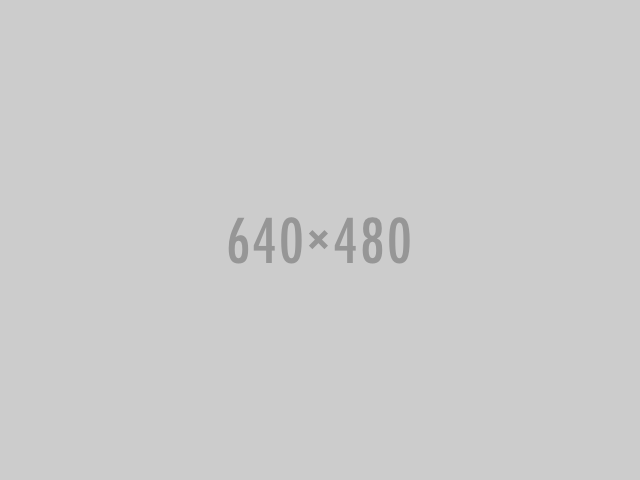
\includegraphics[width=\linewidth,keepaspectratio]{data/chapter-1/placeholder.png}
\caption{示例图片}
\label{figure:sample}
\end{figure}

\section{本文结构安排}

如表~\ref{table:sample}

\begin{table}[!htbp]
\caption{示例表格}
\label{table:sample}
\centering
\begin{tabular}{|c|c|}
\hline
键 & 值 \\
\hline
键 1 & 值 1 \\
\hline
\end{tabular}
\end{table}

    \cleardoublepage
    \chapter{文献综述/技术路线}

\section{第一节}

\section{本章小结}



    \cleardoublepage
    \chapter{研究方案/我做的工作}

\section{第一节}

\section{本章小结}



    \cleardoublepage
    \chapter{实验结果}

\section{第一节}

\section{本章小结}



    \cleardoublepage

    \renewcommand{\thechapter}{}
    \bibliographystyle{data/gbt7714-2005}
\bibliography{data/bibliography}
\addcontentsline{toc}{chapter}{\bibname}

    \cleardoublepage

    \chapter*{致谢}
\addcontentsline{toc}{chapter}{致谢}
\markright{致谢}

待写。

    \cleardoublepage
  }

  {
    \backmatter

    \pagestyle{empty}

    {
  \setlength{\parindent}{0em}
  \linespread{1}

  \vspace*{-2.2em}

  {
    \centering
    \songti\erhao\bfseries
    本科生毕业论文(设计)任务书 \par
  }

  \vspace{2.1em}

  {
    \songti\xiaosi\bfseries
    一、 \; 题目 \; \underline{\makebox{\zjutitlec}}

    \vspace{1.1em}

    二、 \; 指导教师对毕业论文(设计)的进度安排及任务要求

    \vspace{15.5em}

    \hfill 起讫日期 \hspace{2em} 年 \hspace{1em} 月 \hspace{1em} 日 \; 至 \hspace{2em} 年 \hspace{1em} 月 \hspace{1em} 日

    \vspace{1.3em}

    \hfill 指导教师(签名) \; \underline{\hspace{4em}} \; 职称 \; \underline{\hspace{4em}}

    \vspace{2.35em}

    三、 \; 学院审核意见

    \vspace{13.95em}

    \hfill 负责人(签名) \; \underline{\hspace{4em}}

    \vspace{1.3em}

    \hfill \hspace{2em} 年 \hspace{1em} 月 \hspace{1em} 日 \par
  }
}

    \cleardoublepage

    {
  \setlength{\parindent}{0em}
  \linespread{1}

  \vspace*{-2.1em}

  {
    \centering
    \songti\xiaoer\bfseries
    毕~~业~~论~~文~~(设~~计)~~考~~核 \par
  }

  \vspace{1.1em}

  {
    \songti\sihao\bfseries
    一、\; 指导教师对毕业论文(设计)的评语 \par
  }

  \vspace{13em}

  {
    \songti\xiaosi\bfseries
    \hfill 指导教师(签名) \; \underline{\hspace{5em}}

    \vspace{0.1em}

    \hfill \hspace{2em} 年 \hspace{1em} 月 \hspace{1em} 日 \par
  }

  \vspace{0.7em}

  {
    \songti\sihao\bfseries
    二、 \; 答辩小组对毕业论文(设计)的答辩评语及总评成绩:
  }

  \vspace{14.7em}

  {
    \renewcommand{\arraystretch}{1.5}
    \songti\xiaosi\bfseries
    \hfill \begin{tabular}{|c|m{4.1em}|m{4.1em}|m{4.1em}|m{9.1em}|c|}
      \hline
      成绩比例 & {\centering 开题报告 \\ 占(20\%)} & {\centering 外文翻译 \\ 占(10\%)} & {\centering 中期检查 \\ 占(10\%) } & {\centering 毕业论文(设计) \\ 质量及答辩占(60\%)} & 总成绩 \\
      \hline
      分值 & & & & & \\
      \hline
    \end{tabular} \par
  }

  \vspace{2em}

  {
    \songti\xiaosi\bfseries
    \hfill 答辩小组负责人(签名) \; \underline{\hspace{5em}}

    \vspace{0.1em}

    \hfill \hspace{2em} 年 \hspace{1em} 月 \hspace{1em} 日 \par
  }
}

    \cleardoublepage
  }

\end{document}
